\documentclass[a4paper]{article}
\usepackage{geometry}
\usepackage{multicol}
\usepackage{setspace}
\usepackage{listings}
\usepackage{graphicx}
\usepackage{algorithm}
\usepackage{algpseudocode}
\usepackage{amsmath}
\usepackage{amssymb}
\usepackage{multicol}
\usepackage{float}
\DeclareGraphicsExtensions{.eps,.ps,.jpg,.bmp}
\usepackage{xcolor}
%\setlength{\parskip}{0.5\baselineskip}
\geometry{left=3.0cm,right=2.0cm,top=1.5cm,bottom=2.0cm} 
\title{\textbf{Algorithmn HW7}}
\author{5140379032 JIN YI FAN}
\date{}
\begin{document}
\maketitle
\begin{spacing}{1.3}
%\begin{multicols}{2}

\section*{Problem 8.16}
Just change the RELAX part to store the best predecessor of the vertex, 
\\and later we can find the shortest path iterately.
\begin{algorithmic}[1]
\Procedure{Relax}{$u,v$}
\If{$d[v]>d[u]+w(u,v)$}
\State $d[v]\gets d[u]+w(u,v)$
\State $pred[v]\gets u$
\EndIf
\EndProcedure
\end{algorithmic}

\section*{Problem 8.19}
\begin{multicols}{2}
\begin{figure}[H]
    \centering
    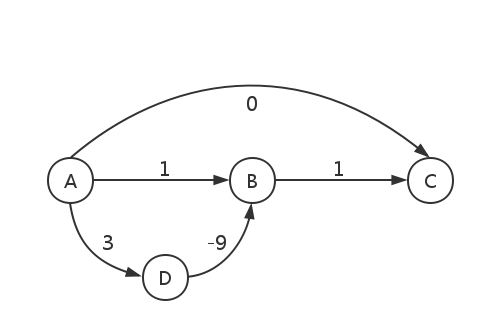
\includegraphics[width=6cm]{dij.png}
\end{figure}
Considering this case, Dijkstra works like this:
\\(1) Starting from $A$, set $d(A)=0$ and $d(others)=+\infty$;
\\(2) $A$ out, set $d(B)=1$, $d(C)=0$ and $d(D)=3$;
\\(3) $C$ out, with no successor edge;
\\(4) $B$ out, with no change ($1+1>0$);
\\(5) $D$ out, updating $d(B)=-6$, then terminate.
\end{multicols}
\noindent Obviously, $d(C)$ should be $-5$ instead of $0$ in this case, which shows Dijkstra does not work in this case.

\section*{True or False}
(a) \textbf{False}, orignally it's $s\rightarrow m\rightarrow n\rightarrow t$ but after modification it will be $s\rightarrow t$
\begin{multicols}{2}
\begin{figure}[H]
    \centering
    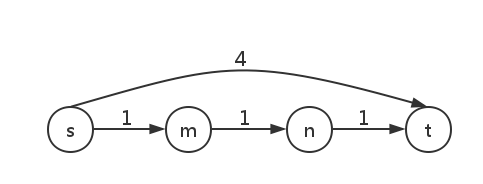
\includegraphics[width=7cm]{c1.png}
\end{figure}
\begin{figure}[H]
    \centering
    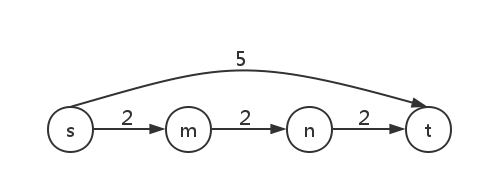
\includegraphics[width=7cm]{c1-2.png}
\end{figure}
\end{multicols}

\begin{multicols}{2}
\noindent(b)\textbf{False}, in the DAG on the right, Dijkstra starting at $m$ definitely won't pick vertexes as any of the topological orders.
\begin{figure}[H]
    \centering
    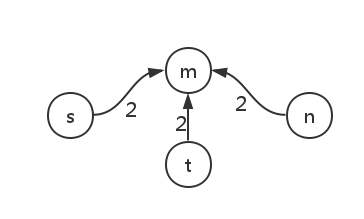
\includegraphics[width=5cm]{c2.png}
\end{figure}
\end{multicols}

\noindent(c)\textbf{False}, because in that case, the short path would be either \textbf{(1)}modified to other path-that won't change-or \textbf{(2)}remain the same path-that will increase the short path by exactly $x$
\\\\\noindent(d)\textbf{True}, because Bellman-Ford will search every possible edge for every vertex regardless of the order, so it will update later if there is some negative value.


\section*{Paths in DAG}
\begin{algorithmic}[1]
\Require a DAG $G=(V,S)$
\Ensure the number of paths in $G$
\Procedure{CountPath}{$G$}
\State topologically sort $G.V$
\State $p[s]\gets 1$, $p[$other $v\in G.V]\gets 0$\Comment{$p[]$ stores the number of paths}
\For{each vertex $i$ in topological sorted sequence}
\For{each vertex $j$ connected with $i$}
\State $p[j]\gets p[j]+p[i]$\Comment{The last element will be the total number of paths}
\EndFor
\EndFor
\EndProcedure
\end{algorithmic}
We can have the relationship as follows:
\\$initial(u)=$ $u$ is the last element in topo order? $1:1+\sum\limits_{(u,v)\in E}$ 
\\$path(u)=initial(u)+\sum\limits_{(u,v)\in E}path(v)$ 
\\Since $path(u)$ and $initial(u)$ can be computed in linear time, the algorithm takes $O(V+E)$ time

\section*{Shortest path tree}
%\end{multicols}
\begin{algorithmic}[1]
\Require directed graph $G=(V,E)$, a tree $T=(V,E')$, $s\in V$ and $E'\in E$
\Ensure whether $T$ is the shortest-path tree of $G$ starting with $s$
\State $Q\gets [s]$
\While{$Q$ is not empty}\Comment{travel the tree}
\State $u=Q.pop()$\Comment{$Q$ is a priority queue}
\For{each edge $(u,v)\in E'$}
\State $d[v]=d[u]+w(u,v)$\Comment{$d[]$ keeps the shortest paths}
\State $Q.push(v)$
\State remove $(u,v)$ from $E'$
\EndFor
\EndWhile
\For{each edge $(u,v)\in E$}\Comment{check in the graph whether it is shortest}
\State $temp\gets d[v]$
\State \Call{Relax}{$u,v$}\Comment{compare the value before and after Relax}
\If{$temp\neq d[v]$}
\State \textbf{return} $False$
\EndIf
\EndFor
\State \textbf{return} $True$
\end{algorithmic}
\end{spacing}
\end{document}

